\documentclass[progress]{cmpreport}
\usepackage{natbib}
\usepackage{graphicx}
\usepackage{wrapfig}
\usepackage{paralist}
\usepackage{outlines}
\usepackage{booktabs}
\usepackage{appendix}
\graphicspath{ {./} }

\title{Third Year Project: Progress Report}
\author{Matthew Taylor}
\registration{100151729}
\supervisor{Dr Rudy Lapeer}
\ccode{CMP-6013Y}

\begin{document}

\maketitle

\begin{section}{Introduction}

\subsection{Aim of the project}
The project aims to implement a first person video game which uses procedural generation (PCG) to provide a novel and interesting game experience. The project will explore the technical aspects of using PCG as a core feature of a game, specifically, implementation and performance. 

It will focus on real-time procedural level generation and providing a compelling, dynamic level structure.

\subsection{Motivation}
Procedural generation is not a new field, especially in video games, but there are interesting areas that are seldom explored.

The motivation behind the project's aims are to explore new and interesting concepts, namely, using PCG as a core feature in a game and using real-time procedural generation to provide an interesting experience.
   
\end{section}

\begin{section}{Issues and problems}

\subsection{Designing 3D games}
Designing 3D games and the assets required to populate the levels created could take a long time, especially if much of the functionality is created from scratch. To enable the project's aims to be achieved in a realistic timeframe, the Unity game engine was chosen. This tool enables relatively rapid production 3D game enviroments, supporting the design of assets and enabling quick prototyping of ideas. Unity supports the use of C\# as a scripting language to program game features in. It also provided a lot of documentation, which was useful in learning the framework and the systems it provides. Much of the initial stages of the project focussed on learning Unity.

\subsection{Performance}
How a game performs is critical to it's success, even at a basic level. If the game cannot be played in a sustainable framerate on common hardware, it could be considered a techncial failure. The prototype stage considered performance at every aspect.

\subsection{Evaluation of success}
A key issue with a project of this type is how success is evaluated. There are a few obvious candidates, which I will list, along with some more subtle intepretations of the projects success.

\subsubsection{Performance}
As alluded to previously, performance is one of the key components of the projects success. Performance will be measured in a few ways:
\begin{itemize}
    \item{Frame rate}
    \item{Initial loading time}
    \item{Smooth level re-generation (no jitter when level changes behind player)}
\end{itemize}

\subsubsection{Convincing levels}
The levels must appear convincing. This is difficult to quantify, but nevertheless is an important attribute. The levels (at least in the initial design) will be mazes generated in a grid, with the grid sections subdivided in different ways.

This could easily create a boring level, where the grid pattern is discernable and the rooms are boring and procedural to traverse. Successful generation of levels will avoid these issues.

\end{section}

\begin{section}{Design and planning}

\subsection{Implementation methodology}
The project development operates under an Agile methology. Agile does not require that all requirements (or "user stories") are defined up front, instead it is encouraged that they are developed and refined during the lifecycle of the project.

The project itself is divided into Agile "sprints". It was decided to deliver a sprint every two weeks, as this fit with the development time given to the project and providing updates to the project supervisor.

While all the stories were not required at the outset, as part of the planning, it was decided to plot rough timescales against Agile "epics". These epics provide a high-level view of functionality and are detailed in Table \ref{tab:epics} on page \pageref{tab:epics}.

The epics also contain very high-level user stories, which provide a little more detail. These were decided at the project outset, then refined during development. Before any user story can be developed, it is required that more detailed requirements are written. These are then recorded and tracked on Trello. 

\subsection{Implementation plan}

With the high-level design documented in the epics, planning of these epics against timescales was required. This timeline plan is visible in \ref{fig:gantt1} on page \pageref{fig:gantt1}. Progress was then tracked against this Gantt chart to ensure that progress was being made and that the project could be achieved as planned.

\subsection{UML}

As the project began, a UML diagram was designed to provide a high level framework to work towards. Unity provides some pre-defined structure, in that all game objects must be part of a Scene object to work. Aside from this, Unity does not prescribe a lot of structure, so having a UML design to begin with was useful. The initial UML design can be seen in Figure \ref{fig:uml1} on page \pageref{fig:uml1}.




\subsection{Requirements and prioritisation}

\subsection{Design}
\subsubsection{Guaranteed path generation}
The first part of the design to be implemented required a guaranteed path through a maze to be generated. This was achieved by using a random walk - a stochastic process implmented in two dimensions to provide a definite route through the maze.

The random walk is implemented using an agent based approach. The agent can choose from three random directions to travel in - left, right or down. These probabilities are detailed in Table \ref{tab:probdirs}.

\begin{table}[h!]
    \centering
    \begin{tabular}{ |c|c|c| }
    \hline
    Left & Right & Down \\ 
    \hline
    40\% & 40\% & 20\%\\ 
    \hline
    \end{tabular}
    \caption{A table showing probability of direction random walk agent will take}
    \label{tab:probdirs}
    \end{table}

This skewed probability distribution encourages the path generating agent to meander left and right more than moving down, generating a path that is longer and doubles back on itself more.



\end{section}

When the agent has chosen a valid direction, it randomly selects a valid tile. To aid in creating an interesting maze, the agent can choose from a variety of pre-made tiles with varying exits. For example, it may choose to generate a room with only left and right openings, or a tile with openings on the left, right and down-facing aspects. 

The agent has methods of checking where it has been and where it is going next, so that it picks valid tiles that have openings in the directions it has come from and intends to go.

The agent is given bounds and restrictions while it is performing the random walk. These bounds ensure the generation does not stray too far left or right. When the agent reaches the lowest down-bound, it stops generating the level and spawns the level's goal in the final tile it generated.

These bounds are adjusted by parameters, which aid in development and testing and can be adjusted based on performance or desired level size.



\begin{section}{Evaluation of progress}
- Changes to aims/scope/work plan
\end{section}






\bibliography{sources}

\newpage

\appendix

\begin{section}{Gantt charts}

\begin{wrapfigure}{l}{0.5\textwidth}
    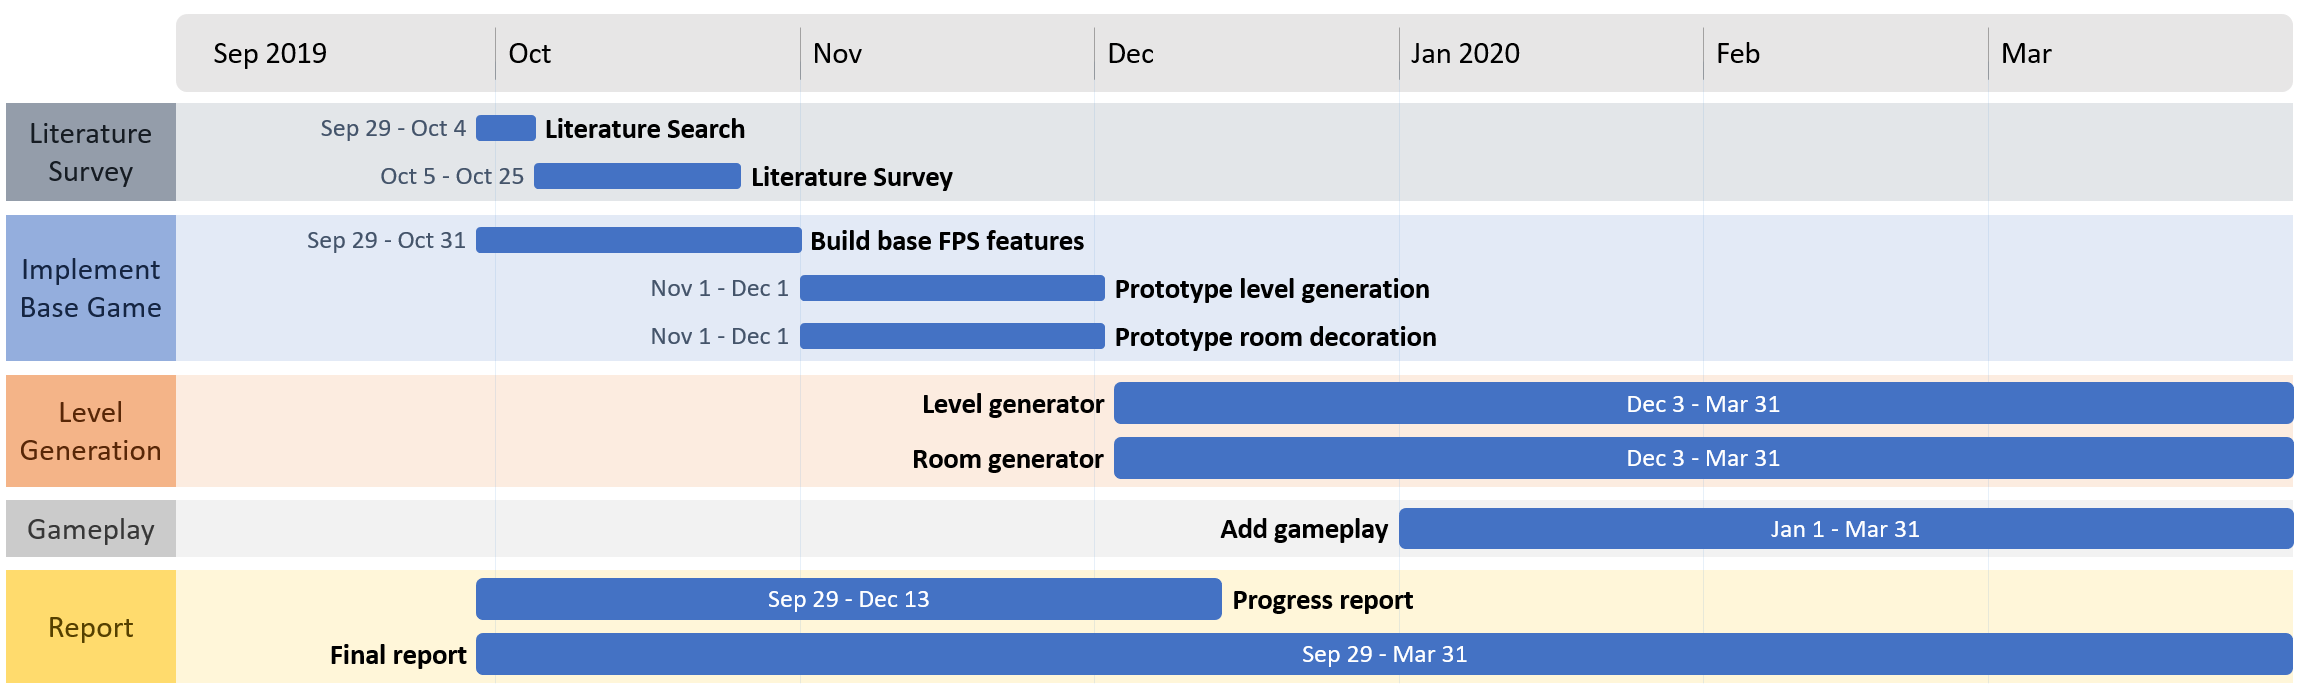
\includegraphics[width=\textwidth,height=0.9\textheight,keepaspectratio]{img/gantt-original.png}
    \caption{Gantt chart of original plan}
    \label{fig:gantt1}
\end{wrapfigure}

\end{section}

\begin{section}{Diagrams}

\begin{wrapfigure}{h!}{0.5\textwidth}
    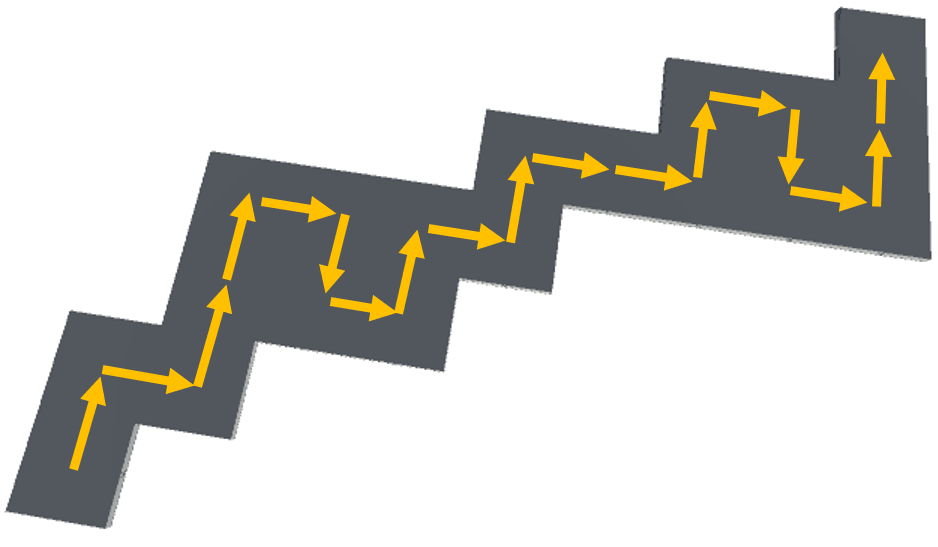
\includegraphics[width=6cm]{img/1-maze.png}
    \caption{A top-down view of the guaranteed path generation}
    \label{fig:pathgen}
\end{wrapfigure}

\begin{wrapfigure}{h!}{0.5\textwidth}
    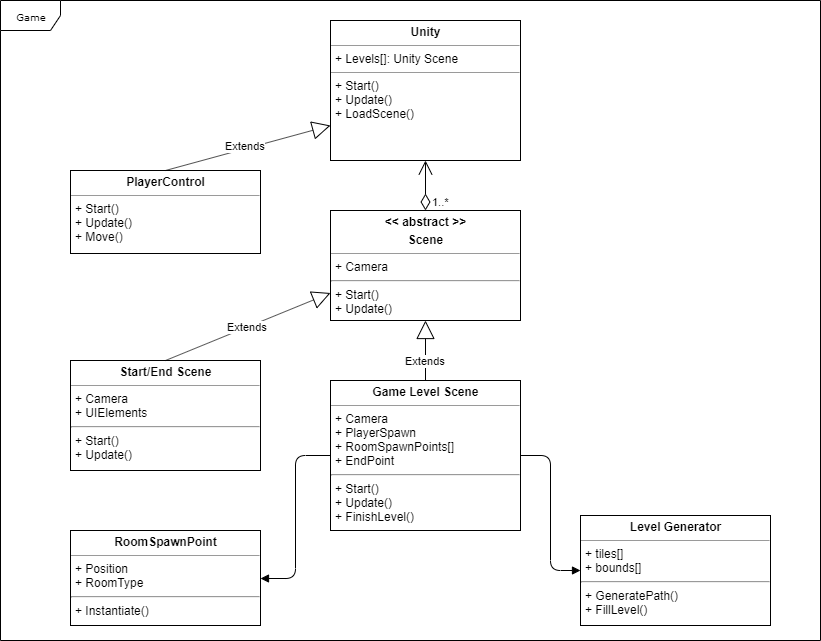
\includegraphics[width=\textwidth]{img/uml1.png}
    \caption{Initial UML diagram}
    \label{fig:uml1}
\end{wrapfigure}

\end{section}

\begin{section}{Tables}

% epic/story table
\begin{table}[]
    \resizebox{\textwidth}{!}{%
    \begin{tabular}{@{}ll@{}}
    \toprule
    \multicolumn{1}{l|}{\textbf{Epic}} & \textbf{Stories} \\ \midrule
    \multicolumn{2}{l}{Build base "first person" 3D game features} \\
     & Provides a basic level design \\
     & Proves the concepts of vision and movement \\ \midrule
    \multicolumn{2}{l}{Prototype level generation} \\
     & Prove a method of generating a guaranteed path through a maze \\
     & Prove a method of filling in non-guaranteed paths through the maze \\ \midrule
    \multicolumn{2}{l}{Prototype room generation} \\
     & Prove a method of generating room interiors \\
     & Room generation must not interfere with guaranteed path \\ \midrule
    \multicolumn{2}{l}{Prototype level re-generation} \\
     & Design method to procedurally re-generate level sections \\ \midrule
    \multicolumn{2}{l}{Add gameplay elements} \\
     & Decide on how level is finished by the player \\
     & Provide some interest and threat when playing \\
     & Provide means of assisting navigation \\ \midrule
    \multicolumn{2}{l}{Implement final designs} \\
     & Use non-prototype textures \\
     & Ensure performance meets goals \\ \bottomrule
    \end{tabular}%
    }
    \caption{Agile-style epics and associated user stories}
    \label{tab:epics}
\end{table}

\end{section}

\end{document}
